\section{Architecture logicielle}
	\label{section:archi}

L'étude d'ADTool a mis en évidence des limitations en ce qui concerne l'analyse des arbres. Afin d'y remédier, de nouvelles fonctionnalités seront implémentées. Ces dernières se décomposent en deux parties : celles qui apportent une véritable plus-value pour l'analyse des arbres, et celles qui facilitent le travail d'édition d'arbres. 

Le projet aboutira donc sur la création d'un nouveau logiciel nommé \glasir{} qui contiendra les nouvelles fonctionnalités d'analyse. Il encapsulera une version améliorée d'ADTool, qui sera son éditeur d'ADTrees. Deux raisons ont motivé la décision de créer un nouveau logiciel. Tout d'abord, cela permet de séparer l'analyse et l'édition des ADTrees, afin d'avoir des logiciels dédiés à leur tâche. Deuxièmement, cette solution permet d'utiliser des technologies différentes de celles d'ADTool, enrichissant ainsi notre formation. La {\sc Figure}~\ref{fig:architecture_Glasir} montre comment ADTool sera intégré dans \glasir{}, ainsi que les modules qui seront développés. % à comparer avec la version précédente sur github

	\begin{figure}[h!]
		\centering
			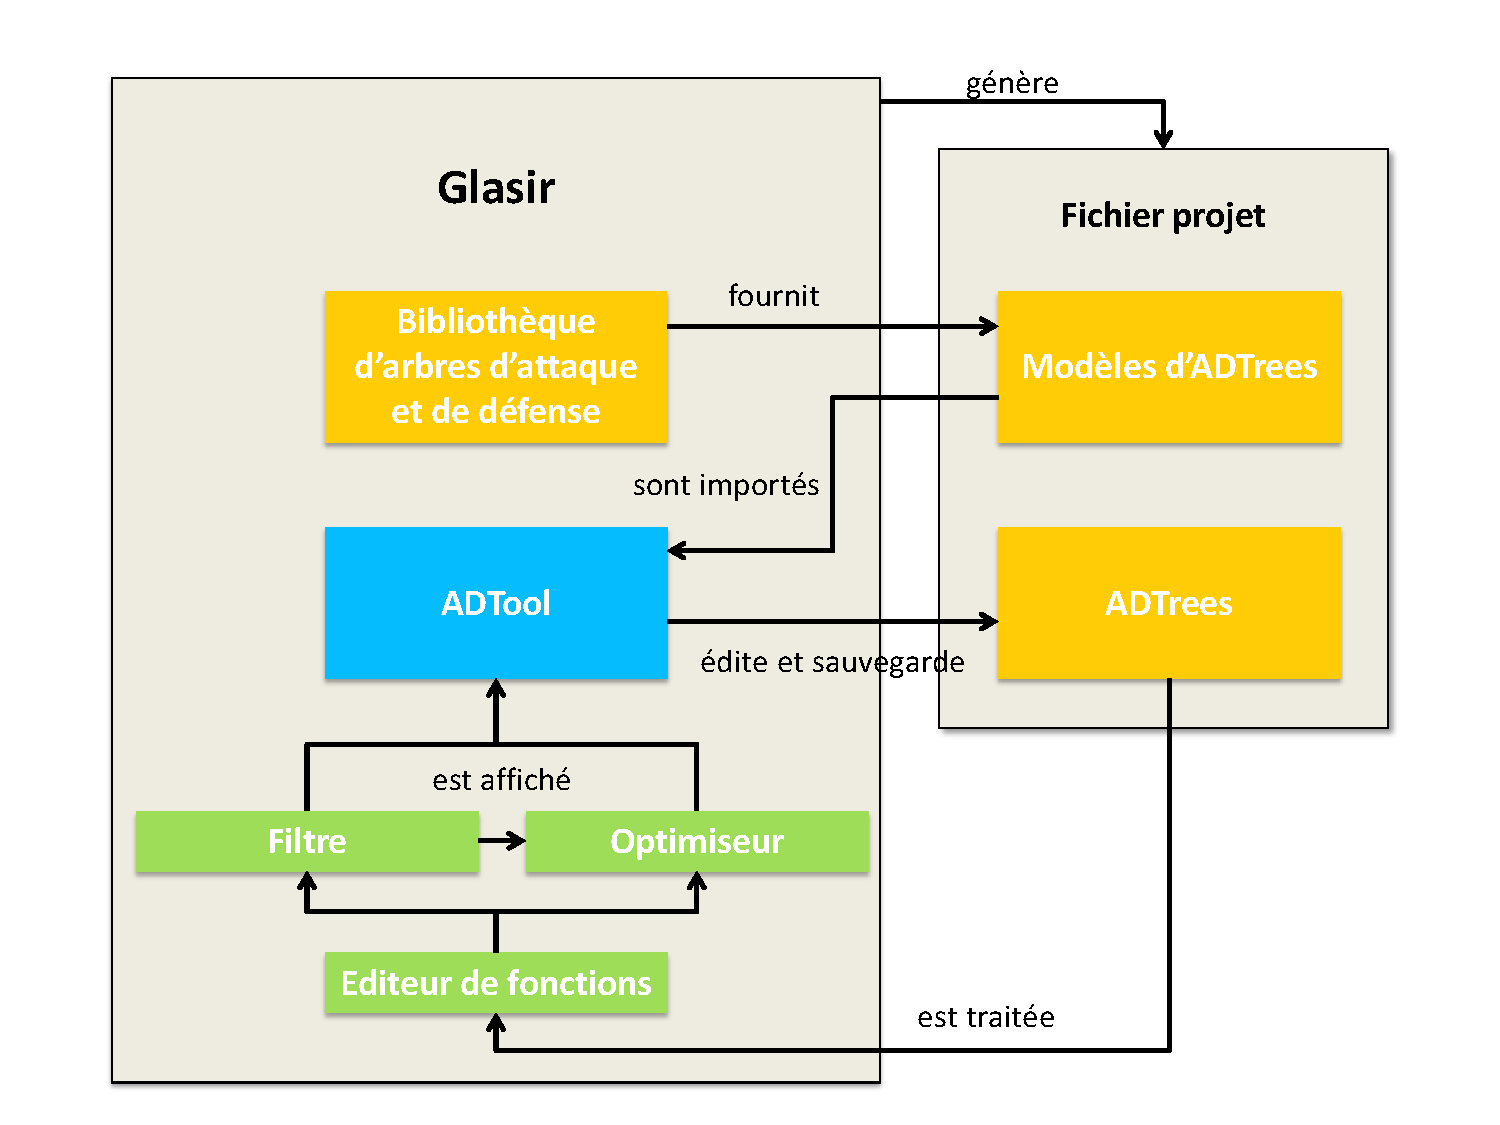
\includegraphics[width=0.8\textwidth]{figure/archiGlasir.pdf}
		\caption{Architecture du logiciel \glasir{}.}
		\label{fig:architecture_Glasir}
	\end{figure}

Comme illustré sur la {\sc Figure}~\ref{fig:architecture_Glasir}, \glasir{} est constitué d'une bibliothèque d'ADTrees, d'ADTool et des nouvelles fonctionnalités d'analyse. L'expert réalisant un projet d'analyse à l'aide de \glasir{} utilisera des fichiers projets. Ils contiennent les ADTrees du projet en cours ainsi que les modèles génériques d'ADTrees que l'expert a jugés utiles pour son projet. Ceux-ci proviennent de la bibliothèque d'ADTrees de \glasir{}.
	
Lors de la création d'un projet quelconque, \glasir{} commence par créer le fichier projet correspondant. L'expert va alors créer ou modifier ses ADTrees grâce à ADTool. Les modèles de la bibliothèque d'ADTrees utilisés dans le cadre du projet seront également sauvegardés dans le fichier projet, pour gérer leurs éventuelles modifications sans impacter la bibliothèque d'arbres génériques de \glasir{}. L'expert pourra alors définir ses paramètres de synthèse avec l’\emph{Éditeur de fonctions}, filtrer les arbres grâce au module \emph{Filtre} ou encore y chercher le chemin optimal à l'aide de l'\emph{Optimiseur}. La prochaine section détaillera l'implémentation de ces différents modules. 